\documentclass[a4paper, 11pt]{article}
\usepackage{geometry}
\geometry{letterpaper, margin=1in}
\usepackage{amsmath}
\usepackage{amssymb}  
\usepackage{amsthm}
\usepackage{ulem} 
\usepackage{graphicx}
\graphicspath{ {images/} }
\usepackage{tikz} 
\begin{document}
%Header-Make sure you update this information!!!!
\noindent
\large\textbf{Complex Analysis - MTH 483} \hfill \textbf{John Waczak} \\
\normalsize Day 9 \hfill  Date: \today \\

\subsubsection*{Complex Curves (paths)} 
\textbf{Definition:} A curve (path) in $\mathbb{C}$ is a continuous function $\gamma:[a,b]\rightarrow \mathbb{C}$. The real numbers have an orientation (from negative to positive). This gives curves a direction in $\mathbb{C}$, beginning at $\gamma(a)$ and ending at $\gamma(b)$. \\ 

\noindent\textit{A few examples:} $\gamma:[0,2]\rightarrow \mathbb{C}$, s.t. $\gamma(t) = (1+2i)t$. This is the parametrization of a straight line. \\
	\begin{figure}[!hbt]
		\centering
		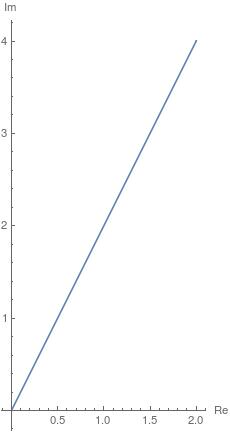
\includegraphics[width=0.35\columnwidth]{straightLine}
		\caption{$\gamma(t) = (1+2i)t$}
	\end{figure}

\noindent In general, to parametrize the \textbf{line segment} from $z_1$ to $z_2$ use: $\gamma(t) = (1-t)z_1 + tz_2$ where $\gamma:[0,1]\rightarrow\mathbb{C}$. \\


\noindent Now lets let $\gamma:[0,1]\rightarrow\mathbb{C}$ s.t. $\gamma(t) = t +it^2$. This is a parametrization of the graph $y(t) = t^2$. \\
	\begin{figure}[!hbt]
		\centering
		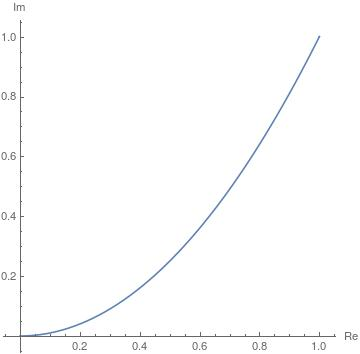
\includegraphics[width=0.35\columnwidth]{parametricParabola}
		\caption{$\gamma(t)=t+it^2$}
	\end{figure}
\pagebreak 

\noindent Here's a circle: $\gamma:[0,2\pi]\rightarrow\mathbb{C}$ by $\gamma(t)=3+2e^{it}$. \\
	\begin{figure}[!hbt]
		\centering
		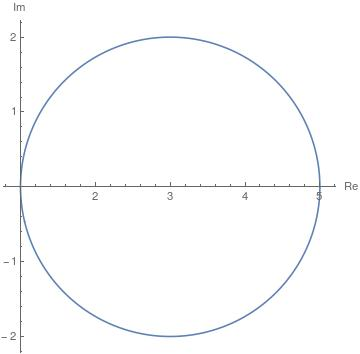
\includegraphics[width=0.35\columnwidth]{parametricCircle}
		\caption{$\gamma(t) = 3 + 2e^{it}$}
	\end{figure}

\noindent Thus in general we have that a \textbf{Circle} of radius $r$ centered at $z_0$ is given by: $\gamma(t) = z_0 + re^{it}$ This parametrization is \textbf{positively oriented} i.e. counterclockwise. For negative orientation, let $t \mapsto -t$. \\

\subsubsection*{Properties of curves in $\mathbb{C}$} 
\textit{Remark:} All curves can be assumed to be piecewise differentiable for finitely many jumps... i.e. only finitely many sharp corners.\\

\noindent\textbf{Definition} The derivative of a complex curve $f(t)$ is accomplished componentwise i.e. if $f(t) = x(t)+iy(t)$ then $f'(t) = x'(t)+iy'(t)$.  \\

\noindent\textbf{Definition} A curve is \textit{Simple} if $\gamma(t)\neq\gamma(tz)$ whenever $a\leq t_1 < t_2 \leq b$, except possible when $t_1=a$ and $t_2=b$. (Curves shouldn't intersect itself except at the end points). \\

\noindent \textbf{Definition} A curve is \textit{Closed} if $\gamma(a) = \gamma(b)$. Think circle. 


\subsubsection*{Complex integration} 
If $g:[a,b]\rightarrow\mathbb{C}$, then we can write $g(t) = x(t) + i y(t)$ for real valued functions $x,y:\mathbb{R} \rightarrow \mathbb{R}$. Then the integral
	\begin{equation*}
		\int_a^b g(t)dt = \int_a^b x(t)dt + i\int_a^b y(t) dt
	\end{equation*}
	
\noindent \textbf{Definition} let $\gamma:[a,b]\rightarrow\mathbb{C}$ be a curve. Let $f(z)$ be a complex valued function which is continuous on the path $\gamma$. Then we define the integral of $f(z)$ over the path $\gamma$ as the following: 
	\begin{equation*}
	\int_\gamma f = \int_\gamma f(z)dz = \int_a^b f(\gamma(t))\gamma'(t)dt
	\end{equation*}
		
\noindent\textit{Example:} $\gamma:[0,1]\rightarrow\mathbb{C}$ s.t. $\gamma(t) = (1-t)+(2+i)t$. Let $f(z)=z^2$. 
	\begin{align*}
		\gamma(t) &= (1-t) +(2+i)t \\ 	
			&= 1+ t + it \\ 
		\gamma'(t) &= 1+i \\ 
		\Rightarrow \int_\gamma f(z)dz &= \int_0^1 f(1+t+it)(1+i)dt \\ 
			&= \int_0^1 (1+t+it)^2(1+i)dt \\ 
			&= (1+i)\int_0^1 (1+(1+i)t)^2dt \\ 
			&= (1+i)\int_0^1 (1+2(1+i)t+(1+i)^2t^2)dt \\
			&= (1+i)\Big[t + (1+i)t^2+\frac{(1+i)^2}{3}t^3\Big]_0^1 \\ 
			&= (1+i)\Big[1 + (1+i_ + \frac{(1+i)^2}{3})\Big]  
	\end{align*}

\noindent \textit{Example} Integrate the function $f(z)=z^2$ over the positively oriented unit circle $\gamma(t) = e^{it}$. 
	\begin{align*}
		\gamma(t) &= e^{it} \\ 
		\gamma'(t) &= ie^{it} \\ 
		\Rightarrow \int_\gamma f(z)dz &= \int_0^{2\pi}(e^{it})^2ie^{it}dt \\ 
			&= i\int_0^{2\pi}e^{3it}dt  \\ 
			&= i\Big[\frac{1}{3i}e^{3it}\Big]_0^{2\pi}
			&= 0
	\end{align*}









	
\end{document}


































